\documentclass[12pt,a4paper]{article}
\usepackage{rmpackages}																% usual packages
\usepackage{rmtemplate}																% graphic charter
\usepackage{rmexocptce}																% for DS with cptce eval

%\cfoot{} 													% if no page number is needed
%\renewcommand\arraystretch{1.5}		% stretch table line height

\begin{document}

\begin{header}
Chapitre 2 -- Solutions aqueuses
\end{header}

\section{Description}

\begin{definition}
Une solution est un mélange liquide homogène constitué :
\begin{itemize}
\item[•] d'un solvant : c'est le constituant majoritaire ;
\item[•] d'un ou plusieurs soluté(s) : ce sont les espèces dissoutes.
\end{itemize}
On parle de solution aqueuse quand le solvant est l'eau.
\end{definition}

\begin{figure}[h]
\center
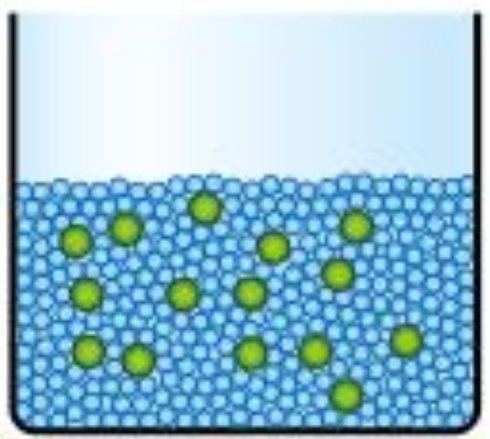
\includegraphics[scale=0.4]{../images/solution_aqueuse.png}
\caption{Description microscopique d'une solution aqueuse.
Les billes bleues représentent les molécules d'eau et les billes vertes représentent le soluté.}
\end{figure}

\begin{remarque}
Le soluté peut être une espèce moléculaire ou ionique.
\end{remarque}
\begin{exemple}
\begin{itemize}
\item[•] le saccharose est un soluté moléculaire ;
\item[•] les ions magnésium Mg\textsuperscript{2+} sont issus d'un soluté ionique.
\end{itemize}
\end{exemple}

\section{Concentration}

\subsection{Concentration massique}

\begin{definition}
La concentration en masse notée $C_\mathrm{m}$ d'un soluté dans une solution est donné par :
\begin{equation}
C_\mathrm{m} = \frac{m_\mathrm{soluté}}{V_\mathrm{solution}},
\nonumber
\end{equation}
où $m_\mathrm{soluté}$ est la masse de soluté dissout et $V_\mathrm{solution}$ le volume total de solution.
\end{definition}

\begin{remarque}
La concentration massique est aussi appelée titre massique, ou encore teneur.
\end{remarque}

\begin{remarque}
Il ne faut pas confondre masse volumique et concentration massique.
\end{remarque}

\begin{figure}[h]
\center
{
\hfill
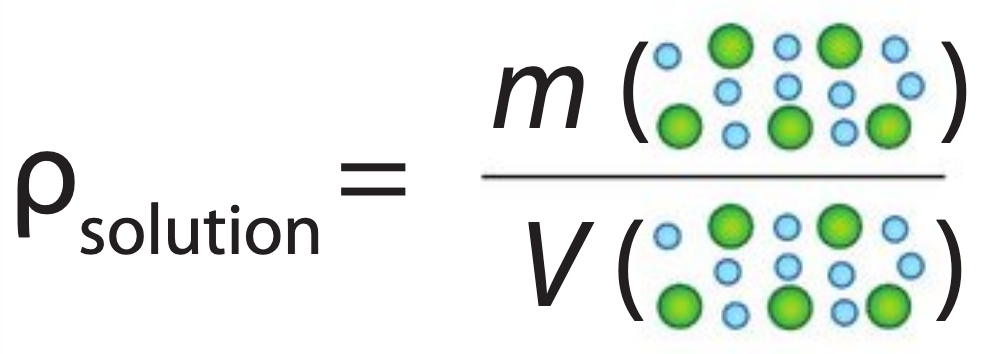
\includegraphics[height=50pt]{../images/difference_rho_t_rho.png}
\hfill
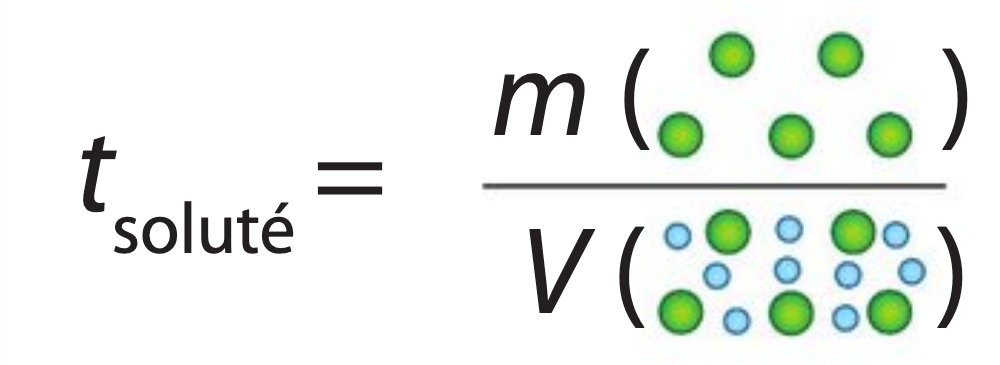
\includegraphics[height=50pt]{../images/difference_rho_t_t.png}
\hfill
}
\end{figure}

\subsection{Solubilité d'un soluté}

\begin{definition}
La solubilité est la masse maximale de soluté qu'il est possible de dissoudre dans un litre de solution.
\end{definition}

\section{Préparation d'une solution aqueuse}

\subsection{Dissolution}

Voir TP dissolution -- Sauvez Maurice et fiche technique dissolution.

\begin{exemple}
\textbf{exercice 6 page 42}

\begin{enumerate}
\item 
\[
C_\mathrm{m} = \frac{m}{V}
\]
En utilisant par exemple la méthode du triangle, on trouve :
\[
m = C_\mathrm{m} \times V.
\]
$m$ s'exprime en grammes (g), $V$ en litres (L) et $C_\mathrm{m}$ en gramme par litre (g/L).

\item 
\[
m = C_\mathrm{m} \times V = 0{,}50 \times 0{,}200 = \unit{0{,}10}{g}.
\]
La masse à peser est $m = \unit{0{,}10}{g}$.
\end{enumerate}
\end{exemple}

\subsection{Dilution}

Voir TP dilution et fiche technique dilution.

\begin{exemple}
\textbf{exercice 20 page 44}

\begin{enumerate}
\item 
\[
t_\mathrm{m} \times V_\mathrm{m} = t_\mathrm{f} \times V_\mathrm{f}
\]
On cherche $V_\mathrm{m}$ donc on divise de chaque côté par $t_\mathrm{m}$ :
\[
V_\mathrm{m} = \frac{t_\mathrm{f} \times V_\mathrm{f}}{t_\mathrm{m}}.
\]
$t_\mathrm{m}$ et $t_\mathrm{f}$ s'expriment en grammes par litre (g/L) et  $V_\mathrm{m}$ et $V_\mathrm{f}$ en litres (L).

\item 
\[
V_\mathrm{m} = \frac{t_\mathrm{f} \times V_\mathrm{f}}{t_\mathrm{m}} = \frac{0{,}10 \times 0{,}200}{0{,}25} = \unit{0{,}080}{L}.
\]
La volume de solution mère à prélever est $V_\mathrm{m}  = \unit{0{,}080}{L}$.
\end{enumerate}
\end{exemple}

\end{document}